\documentclass[../main.tex]{subfiles}

\begin{document}

\chapter{Evaluation}
\label{chap:evaluation}

This chapter evaluates the protocol proposed in \cref{chap:design}.
Besides the verification of the intended functionality in \cref{sec:evaluation-func}, the security and performance of the protocol are investigated in Sections \ref{sec:evaluation-sec} and \ref{sec:evaluation-perf}.
This evaluation verifies that the system requirements given in \cref{chap:requirements} can be fulfilled.

\section{Functionality}
\label{sec:evaluation-func}

This section evaluates the functionality of the designed protocol.
Specifically, the protocol must ensure that the data owner can always access its logs.
The data owner must also be able to share and revoke access to logs.
Please see \cref{functional-requriements} for details about those functional requirements.

To ensure that data owners can always access their logs, the protocol relies on three mechanisms:
First, the monitor must encrypt a new log only for the data owner.
Hence, a log is accessible for the data owner upon creation.
Second, whenever the data owner shares or revokes access to a log, it must include its own identity in the set of authorized users.
Finally, the server must ensure that no other user besides the data owner can modify encrypted logs.
This guarantees that the data owner is always able to download and decrypt its logs.

The protocol is based on hybrid encryption.
This means that the log is encrypted with a symmetric encryption scheme.
The used symmetric key is then encrypted for each intended recipient.
Those encrypted keys are attached to the encrypted log.
This allows the construction of ciphers that can be decrypted by multiple users.
Hence, a data owner can re-encrypt the log for a specific set of users by applying the encryption algorithm.
The specified metadata allows the server to filter logs for the requesting user.
Moreover, the server can ensure that only the specified data owner can update a log.
This effectively enables the functionality to share and revoke access to the log.
Sharing a log is realized by adding additional users to the set of authorized users.
Revoking access to logs requires omitting a user from this set.
Since new key material is generated during encryption, revoked users cannot re-use older decryption keys to access the log.

This analysis shows that the designed protocol fulfills all identified functional requirements.
A data owner can always access its logs and it can share and revoke access to them.
The protocol was included in the existing toolchain within the scope of this thesis.
\cref{sec:toolchain-modifications} investigates the implemented changes.
This integration verifies that the protocol has the intended functionality and can be used in practice.
Moreover, the implemented libraries are tested.
This creates further confidence in their functionality.

\section{Security}
\label{sec:evaluation-sec}

This section investigates the security of the designed protocol.
Three security requirements were identified during requirements engineering (details in \cref{security-requriements}).
Each requirement was motivated by a concrete attack scenario.
In the following sections, the proposed protocol is confronted with those attacks.
They argue why the established security mechanisms resist them.

\subsection{Assumptions}

The security of the protocol relies on three fundamental assumptions.
If one of those assumptions is violated, the protocol is considered insecure.

First, it is assumed that the protocol has access to a secure PKI.
The PKI assigns the identities of users to their public keys via certificates.
The user must have exclusive access to his private keys.
The public keys are distributed via certificates, which are signed by a trusted certificate authority.
If any private key is compromised, the intended E2EE is broken.
A private key is assumed to be compromised if any entity besides the owner of the private key has access to it.

Second, it is assumed that the JOSE standard provides secure encryption and signing algorithms.
Specifically, \verb|A256GCM| and \verb|ECDH-ES+A256KW| must be secure encryption algorithms and \verb|ES256| must be a secure signing algorithm.
This implies that it is computationally infeasible to break those algorithms without knowing the respective keys~\cite{Katz2020}.

Third, the libraries implemented in this thesis rely on language-specific JOSE implementations (details in \cref{sec:implemented-libraries}).
It is assumed that those libraries follow the specifications and definitions of the JOSE protocol.

\subsection{Curious server}
A curious server is a passive attacker that tries to access the logs within the toolchain.
It motivated security requirement S1, which states that only authorized users can access logs.
Recall the attacker Eve who is the database admin of the \emph{Safekeeper} server (details in \cref{security-requriements}).
This section argues why Eve cannot access logs if he was not explicitly authorized.

The protocol enforces that only encrypted data is stored in the database.
Both, the monitor creating a log and the data owner sharing a log must encrypt the data before sending it to the server.
The server only has access to the JWE token created by the encryption algorithm.
This JWE token relies on hybrid encryption:
First, a symmetric key $k$ is randomly generated and the data is encrypted via \verb|A256GCM|.
This is an authenticated\footnote{Note that this authentication does not guarantee the authenticity of the sending user. This is because in a symmetric encryption scheme the authenticity is always bound to the knowledge of the symmetric key. Since multiple receivers might have access to the symmetric key, this authentication only ensures that any of those users generated the cipher. To ensure the authenticity of the sending user, the protocol must include a digital signature.~\cite[315]{Eckert2018}} symmetric encryption algorithm based on AES~\cite{JWA2015}.
Secondly, this symmetric key $k$ is encrypted for each receiver using \verb|ECDH-ES+A256KW|~\cite{JWA2015}.
This key-wrapping algorithm establishes an ephemeral key between two users.
This ephemeral key is finally used to encrypt the symmetric key $k$.
Details about this algorithm can be found in \cref{sec:encrypting}.

To access a decrypted log, the attacker Eve needs to have access to the symmetric key $k$.
This requires him to decrypt any of the encrypted keys attached to the JWE token.
To succeed, Eve must have access to any of the ephemeral keys used to encrypt $k$.
Eve can compute an ephemeral key only if he has access to either the ephemeral private key of the sender or the static private key of the receiver.
However, those private keys must be kept secret.
If Eve wants to decrypt the log, he must either break the encryption algorithms or access a private key.
This, however, contradicts the assumptions.
If Eve can break the encryption, the used encryption algorithm is not secure.
If Eve can access a private key of a user, the PKI is not secure.
This leads to the conclusion that the malicious database admin Eve cannot access decrypted logs.
Only if he was explicitly authorized, he can restore the symmetric key $k$, which allows the decryption of a log.

Note that a curious server has access to the metadata of an encrypted log.
This metadata consists of the identity of the data owner, which ensures only authorized users can update the stored log, and the identities of the recipients, which ensures that the \emph{Safekeeper} can distribute the logs to the correct users.
Although intermediate servers cannot access the log data itself anymore, the metadata yields the information on which users have access to which log.
This information could be subject to a metadata analysis attack~\cite{Greschbach2012,Mayer2016}.
If the underlying single-sign-on server supports pseudonyms for users, however, this attack could be made significantly more difficult.
Pseudonyms could be assigned to the users participating in the system.
Instead of providing a unique identity within the metadata, a random pseudonym of the user could be chosen.
Assuming that the intermediate server cannot link pseudonyms back to users, this would make the metadata analysis pointless.

\subsection{Surreptitious forwarding}
Surreptitious forwarding refers to an attack where a malicious user re-encrypts and forwards a received log for unintended users~\cite{Davis2001}.
Since such attacks must be detected, the security requirement S2 was introduced.
Receivers of encrypted logs must be able to verify that the log was intentionally shared with them.
Recall the attacker described in \cref{security-requriements}.
Alice shares a log with Eve.
This implies that Eve has access to the decrypted data.
Eve, however, does not stick to the protocol and encrypts the received log for Bob.
Bob must be able to detect this fraud because the log he received was not encrypted by the data owner Alice.
This section argues why the designed protocol can detect this attack.

The construction introduced to defend against this attack is the \emph{shared log}.
It is a JWS token that is signed by the creator of the log.
For details see the visualization in \cref{fig:nested-jws}.
A \emph{shared log} contains the log as a nested JWS token.
Moreover, it contains the identity of the creator and the identities of the intended receivers.
Whenever a user successfully decrypts a log, it must verify that the \emph{shared log} is a valid data structure (see \cref{sec:decrypting} for details).
This includes the following three checks.
First, the receiver needs to verify if the \emph{shared log} was signed by the claimed creator.
Second, the receiver then needs to check if the claimed creator is also the data owner of the log. 
Third, the receiver must verify if his identity is specified in the list of intended receivers.
The following consequence is observed from this validation:
The creator specified in the \emph{shared log} must have signed the \emph{shared log}.
The creator specified in the \emph{shared log} must be equal to the data owner.
Thus, the \emph{shared log} is only valid if the data owner has created the signed log.

Eve has two options to forward an encrypted log to the unintended receiver Bob.
First, Eve could manipulate the identity of the data owner.
If he manages to change the identity of the data owner to its own identity, he could correctly sign the \emph{shared log}.
This modification, however, makes his attack pointless.
Eve does not want to introduce faked logs.
He wants to forward existing logs to unintended receivers.
Moreover, this requires Eve to be a valid monitor because only they are allowed to sign logs.
Second, Eve could try to forge the signature of the data owner Alice.
This does not require him to modify the log.
Rather, Eve keeps the existing log and creates a \emph{shared log} that includes Bob as a valid receiver.
He also specifies Alice as the creator of the \emph{shared log}.
This approach requires Eve to create a signature in the name of Alice because Bob will check if the claimed creator signed the \emph{shared log}.
However, this contradicts the assumptions:
To successfully forge a signature, Bob either has access to the private signing key of the data owner or he breaks the signing algorithm.
The former breaks the security of the assumed PKI.
The latter breaks the security of the chosen signing algorithm.

This analysis shows that there is no way for Eve to forward a received log to unintended recipients if those recipients validate the \emph{shared log} correctly.


\subsection{Malicious data owner}
A malicious data owner is a user trying to modify existing logs or create arbitrary new logs.
It then tries to share the forged log with other users in the system.
Security requirement S3 was introduced to defend against this attack.
This section elaborates on how recipients of logs can detect this fraud.

The designed protocol defines a log as a cryptographically signed data structure.
Each log must be signed by a valid monitor.
The protocol also requires the validation of this signature during decryption.
In particular, a receiving user must perform two checks to ensure the validity of the log.
First, the monitor specified within the log must have signed the log.
This requires the receiver to download the public verification key of the claimed monitor.
The receiver can be sure that the log was signed by the private key of the monitor if the verification succeeds.
Second, the receiving user must also validate that the claimed monitor is allowed to create logs.
Otherwise, arbitrary users could sign logs.
This requires the installed PKI to deliver this information, e.g. by encoding it into the certificates of the monitor components.

Consider Eve to be a malicious data owner trying to share a forged log.
First of all, Eve creates his malicious log data.
He then needs to sign this data using the private signing key of the monitor specified in the log.
Otherwise, the recipient would notice that the claimed monitor did not sign the log.
Eve has two options.
First, he could specify his identity and sign the log with his private signing key.
Eve must be a valid monitor because otherwise, the recipient would detect the fraud.
Second, Eve could specify an existing monitor in the log.
This passes the check if the claimed monitor is allowed to create logs.
However, it requires Eve to create a signature in the name of the monitor, which contradicts the assumptions.
Either he needs access to the private signing key of the claimed monitor (insecure PKI) or he needs to break the signing algorithm (insecure algorithm).
Both options are not feasible under the given assumptions.
Thus, a malicious data owner Eve cannot introduce forged logs into the system.

\section{Performance}
\label{sec:evaluation-perf}
This section contains performance evaluations of the provided implementations.
\cref{sec:evaluation-perf-enc} analyzes the encryption duration of the implemented cryptographic libraries.
\cref{sec:evaluation-perf-toolchain} investigates the overhead of the added encryption layer in the \emph{transparency toolchain}.

\subsection{Encryption}
\label{sec:evaluation-perf-enc}
As elaborated in the previous chapters, the designed and implemented protocol is based on hybrid encryption.
Hence, logs can be encrypted for multiple recipients.
The symmetric key $k$, which encrypts the log, must be encrypted for each receiver.
This implies that if a log is shared with $n$ users, the key $k$ must be encrypted $n$ times.
Thus, the encryption duration is assumed to increase linearly with the number of recipients.
This section aims to provide resilient measurements of those costs.

\subsubsection{Methodology}
The encryption times are measured for each library separately (ts-it-crypto, py-it-crypto, and go-it-crypto).
The measurements are implemented as performance tests in each library.
All of them follow the same principles.
The encryption duration is quantified by measuring the passed milliseconds during encryption.
Always the same log data is encrypted.
However, the number of recipients changes during different tests.
For a fixed number of recipients, a test is repeated $100$ times.
The average of those runs is said to be the encryption duration for the number of recipients in the library under test.

The performance tests were executed on a machine running \emph{macOS Monterey} with an \emph{Apple M1} ARM64 CPU and 16 GB RAM.
The Go library was compiled with Go 1.18.3\footnote{\url{https://go.dev/doc/devel/release}}.
The Typescript package was compiled into Javascript using TSC 4.8.3\footnote{\url{https://www.typescriptlang.org/docs/handbook/compiler-options.html}}. 
It was then executed by the Node.js version 18.12.1\footnote{\url{https://nodejs.org/ca/blog/release/v18.12.1/}}, which is built upon the V8 engine 10.2.154.15\footnote{\url{https://v8.dev/}}.
The Python tests were run under Python 3.9.6\footnote{\url{https://python.org/downloads/release/python-396/}} using the CPython\footnote{\url{https://github.com/python/cpython}} interpreter.

\subsubsection{Results}
The results of all three libraries are illustrated in \cref{fig:performance}.
It shows the encryption duration in milliseconds for a different number of recipients.
In general, one can observe that the Go implementation is the fastest library.
This meets the expectations because Go is a compiled language while Python and Typescript are interpreted.
Note that Typescript is compiled into Javascript.
The resulting Javascript code, however, is also interpreted by the V8 engine included in Node.js.
The performance difference between the Python and Typescript implementations is remarkable.
Both rely on the native OpenSSL module installed on the operating system.
Hence all complex cryptographic tasks are computed by pre-compiled libraries.
This improves the performance of both libraries.
The observed speed difference can be explained best when considering the performance differences between the Javascript engine V8 and the CPython interpreter:
The experiments performed by~\cite{Lion2022} indicate that execution times under V8 are on average almost four times faster than under CPython.

For all packages, one can observe a linear growth of encryption times when adding additional recipients.
This meets the expectations because all libraries rely on hybrid encryption.
When adding a new user, the encrypting party must additionally encrypt the secret key for this user.
The encryption for a single receiver in Go takes $0.12ms$.
The encryption for two receivers takes $0.17ms$.
The additional receiver increases the costs by about $0.05ms$ because both runs encrypted the same log.
The same analysis can be done for the Python and Typescript libraries.
While an additional recipient in Python increases the encryption costs by approximately $0.50ms$, the Typescript implementation requires about $0.30ms$ for an additional user.

From the perspective of a user, a system reacts instantaneously if a computation takes less than $100ms$~\cite{Nielson1993}.
In those cases no visual feedback is necessary.
Experiments with the packages show that this threshold is reached in Typescript if encrypting the log for about $330$ users.
The Python implementation reaches the boundary if data is encrypted for $170$ users.
In Go, the encryption for $1500$ recipients takes on average slightly more than $100ms$.
This shows that a data owner can share his logs with up to 170 users without noticing a computation delay during encryption.


\begin{figure}[ht]
    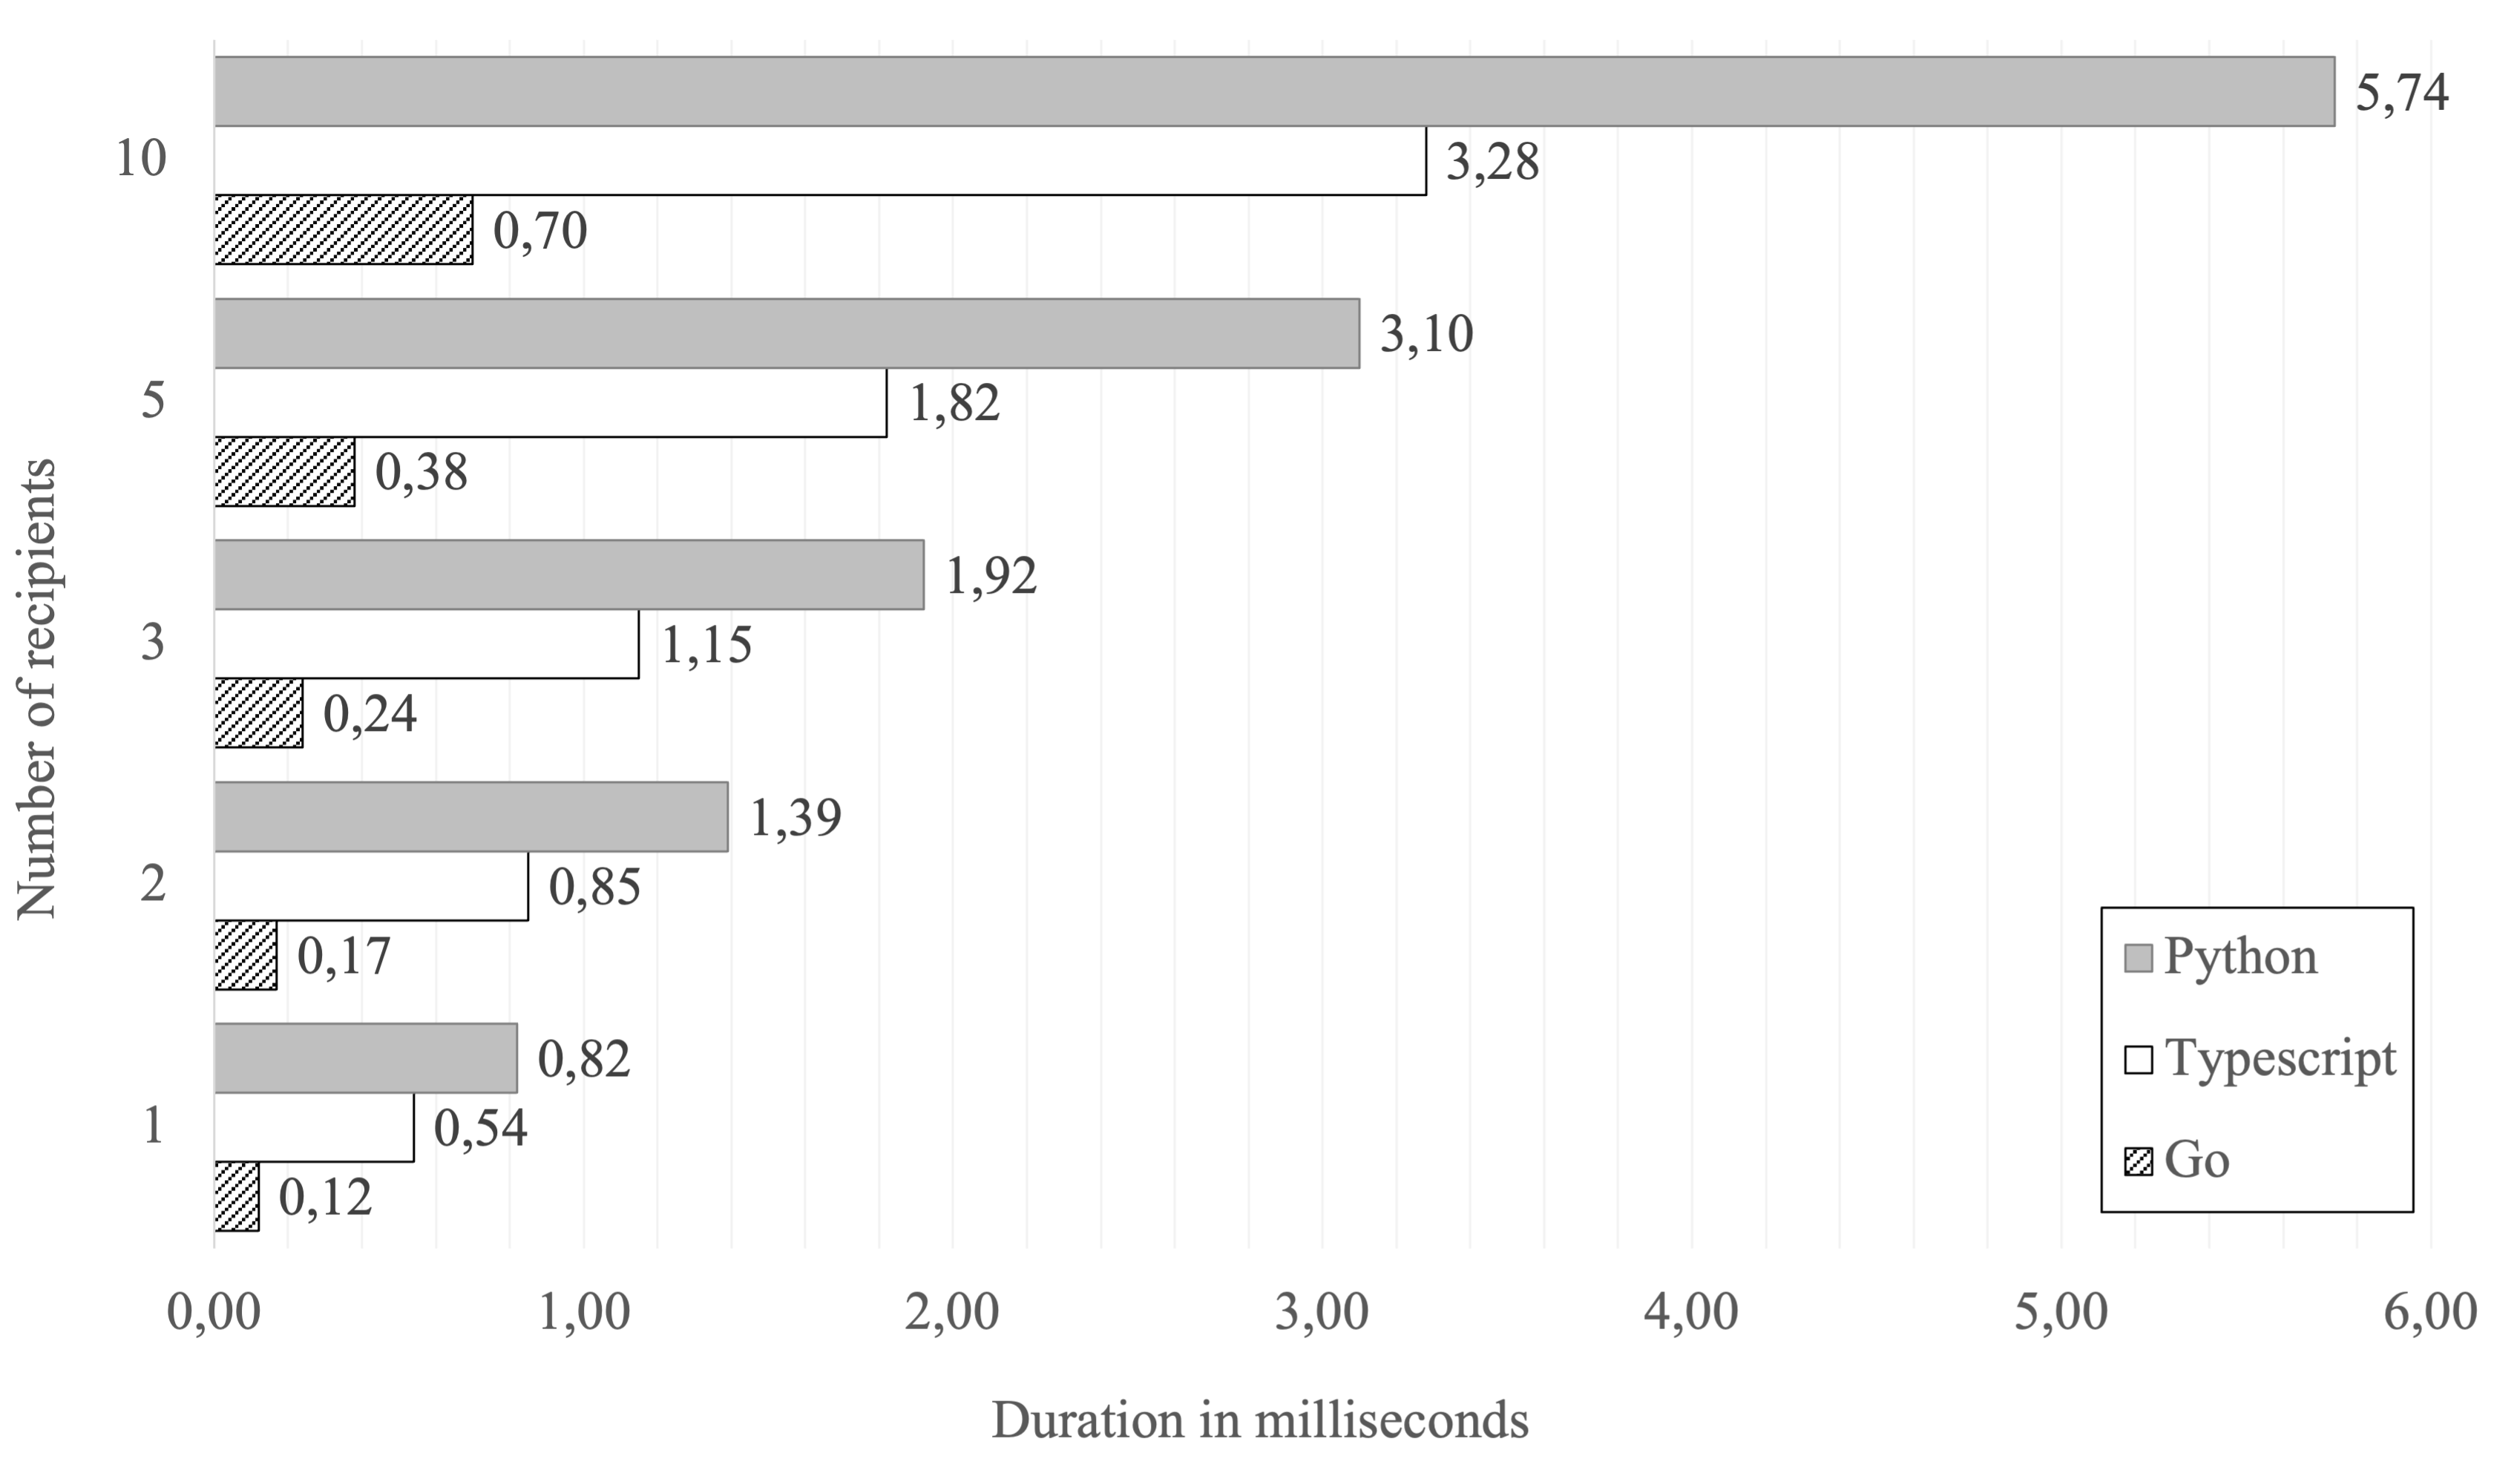
\includegraphics[scale=0.6]{../img/07/performance.png}
    \centering
    \caption[Encryption duration]{This figure visualizes the encryption duration of the different libraries in milliseconds. The same log data was encrypted for a different number of recipients.}
    \label{fig:performance}
\end{figure}

\subsection{Toolchain}
\label{sec:evaluation-perf-toolchain}
The \emph{transparency toolchain} was adopted to support encrypted logs.
Once a user logs in to the \emph{Display} component, all encrypted logs of this particular user are fetched from the \emph{Safekeeper}, decrypted, and visualized.
Compared to the legacy solution, this implementation introduces an additional encryption layer.
It is assumed that this degrades the performance of fetching and visualizing logs because all received logs must be decrypted in the front-end.
This section provides measurements of 
1) the legacy toolchain that does not rely on encryption and
2) the updated toolchain that handles encrypted logs.
Those measurements illustrate the performance differences of the toolchain when encrypted logs are fetched from the server and processed in the front-end.


\subsubsection{Methodology}

The measurements were conducted within the \emph{Display} and the \emph{Safekeeper} component.
They reflect the passed time from starting an API call to fetch logs until those logs are ready for visualization.
This time can be divided into three sections: Database queries, server computation time, and client computation time.
First, the database queries reflect the time the server needs to extract the logs and other information from the database.
Second, the server computation time is the time the server needs to resolve the API call besides the time for querying the database.
For example, the legacy toolchain computes some metadata data over the returned logs and includes this data in the response.
Third, the client computation time is the time needed by the client to process the fetched data until it is available for visualization.
For example, the overview data must be computed by the front-end in the context of encrypted logs.
This is because this metadata can only be calculated once the logs are decrypted.
Moreover, the client computation time includes all tasks that are performed once the API call has finished.
The time for decrypting logs is also part of the client computation time.

The database queries are measured directly within the \emph{Safekeeper} component.
The \emph{Display} component measures the time needed for the entire API call.
To compute the server computation time, the database queries are subtracted from the duration of the entire API call.
The client computation time is measured directly within the \emph{Display} component.

To provide resilient measurements, the database always contains $1000$ logs for the logged-in user.
The number of fetched and visualized logs changes during different tests.
The tests run for $1$, $10$, and $100$ logs.
For a fixed number of logs, a test is repeated $100$ times.
The presented numbers are the averages over all runs.
Each test is run against the legacy toolchain and the updated toolchain.
The tests were executed within the development environment, which was started using \verb|docker-compose|.
They were executed on a machine running \emph{macOS Monterey} with an \emph{Apple M1} ARM64 CPU and 16 GB RAM.


\subsubsection{Results}
\cref{fig:perf-unencrypted} shows the results of the legacy toolchain.
Overall, the toolchain requires on average $142ms$ to fetch a single log, $148ms$ to fetch ten logs, and $243ms$ to fetch one hundred logs.
The server computation time increases when multiple logs are fetched.
This is expected because the server computation time includes the transmission delay over the network.
Furthermore, one can observe that the client computation time is very fast.
The main reason for this lies in the fact that the server performs different pre-computation steps needed to visualize the logs in the front-end.
Hence, the front-end can directly visualize the logs without further computation.
For example, the server fetches metadata from the database to provide the number of logs that were created within a specific tool.
The database queries account for a big portion of the time needed to fetch logs from the server.
There are two reasons for this.
First, the pre-computed data relies on multiple database queries.
Second, the realized database schema requires a database join to resolve the identity of a user to a given access log.
Thus, the measured database query times are higher in the legacy toolchain than in the updated toolchain.
The time needed to query data from the database increases slightly when more logs are loaded from the server.
This is expected since the database must resolve more data if more logs are requested.

\begin{figure}[ht]
    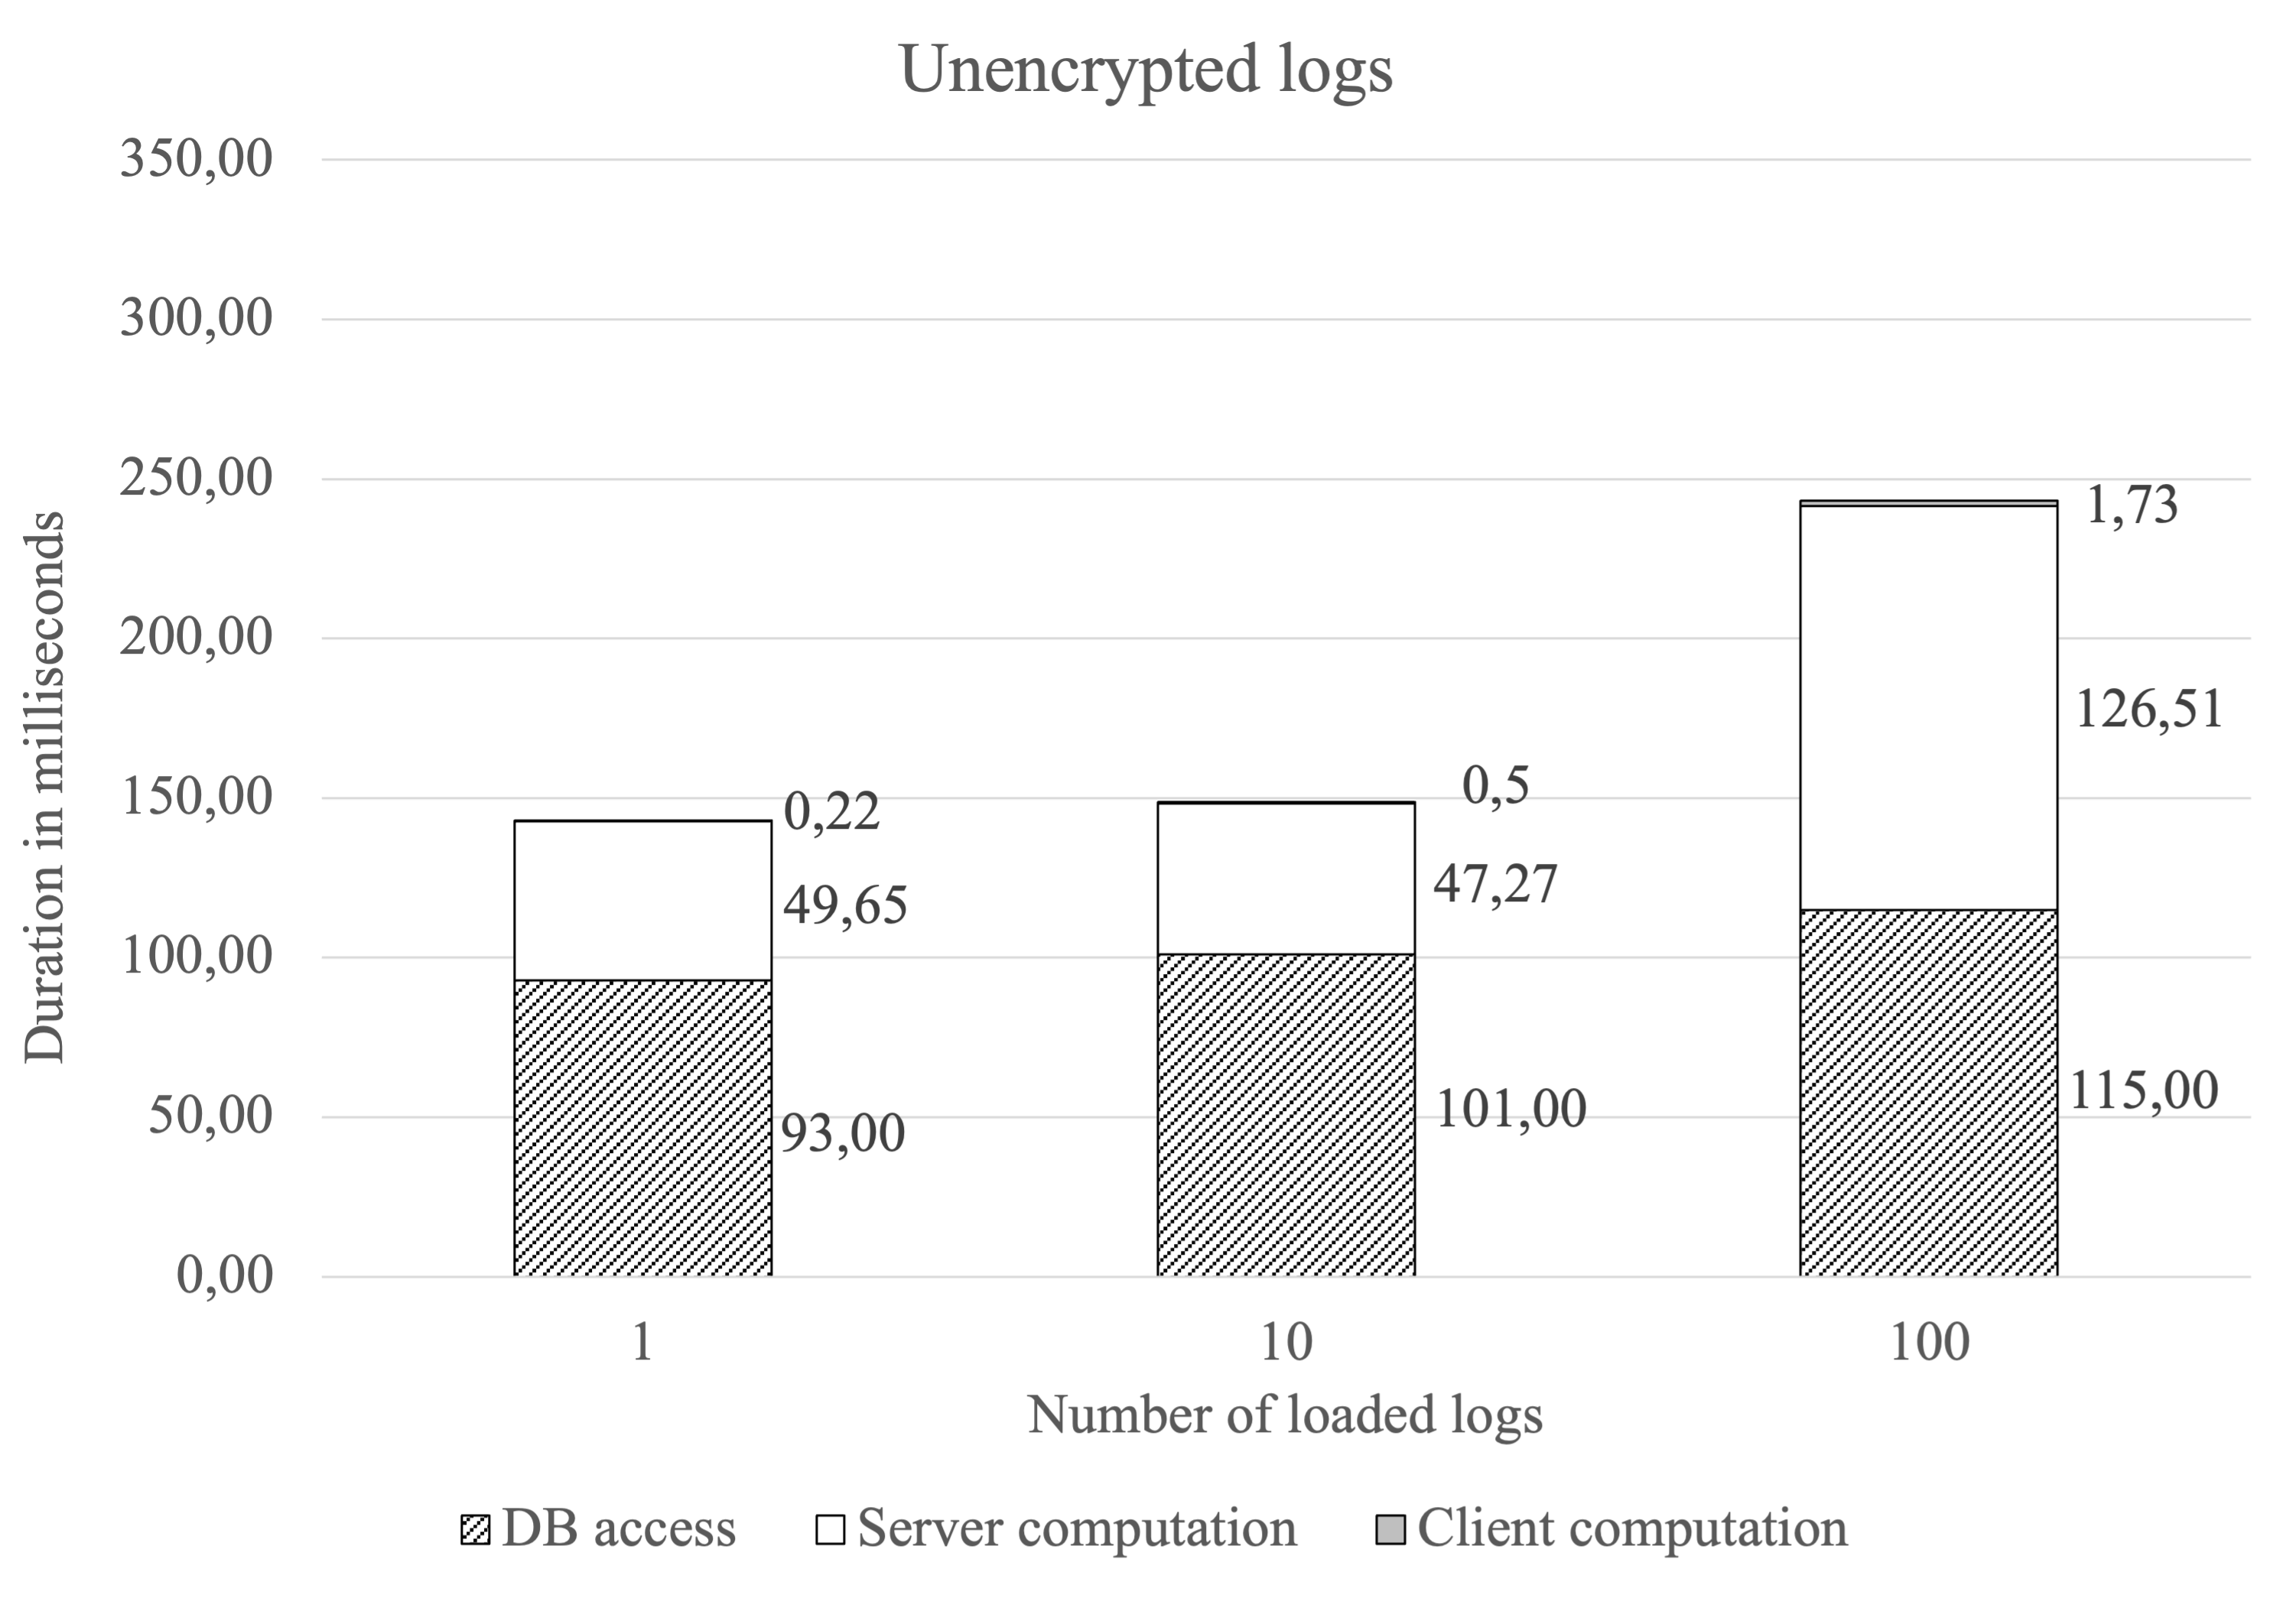
\includegraphics[scale=0.62]{../img/07/unencrypted.png}
    \centering
    \caption[Measurements legacy toolchain]{This figure visualizes the measured times to download and process the logs in the previous toolchain, which maintains unencrypted logs.}
    \label{fig:perf-unencrypted}
\end{figure}

\cref{fig:perf-encrypted} shows the results of the updated toolchain including the encryption layer.
Overall, the updated toolchain requires on average $77ms$ to fetch a single log, $106ms$ to fetch ten logs, and $298ms$ to fetch one hundred logs.
Those results are not expected because for a single log and ten logs the encrypted toolchain is faster than the legacy toolchain.
The reason for this lies in the pre-computation performed by the legacy toolchain, which depends on multiple database queries.
Those pre-computation queries require more time than the decryption of the logs in the updated toolchain.
Moreover, the updated toolchain employs a simplified database design consisting of a single table that stores the encrypted logs.
As described in ~\cref{sec:implemenation-safekeeper}, this table contains two JSON fields.
They could be further improved to support efficient indexed lookups~\cite{Shang2021}.
Querying the logs from this table is more efficient than querying logs in the old database scheme because only a single query without database joins is executed.
Thus, the aggregated duration of all database queries is smaller in the updated toolchain compared to the legacy version.
\cref{fig:perf-encrypted} illustrates that server computation times increase if multiple logs are fetched.
Again, this is expected because it contains the transmission delay of the data sent over the network.
The more data is transferred, the longer the transmission delay.
Compared to the legacy toolchain, the server computation time has increased.
The size of an encrypted log is about $1600$ bytes.
The size of an unencrypted log is $700$ bytes on average.
The updated toolchain must transfer more data than the legacy version because encrypted logs introduce a memory overhead.
Hence, the legacy toolchain requires less server computation time.
Finally, the client computation time is higher in the updated toolchain.
If the client fetches $100$ logs, their processing takes about $114ms$.
Compared to the very short processing times in the legacy version, this is a significant increase.
There are two reasons for this.
First, the received logs must be decrypted.
Second, the decrypted logs are analyzed to provide metadata for the visualization in the front-end.
In the legacy version, this was computed by the server.
Since the log data must be decrypted to compute this metadata, however, this computation was shifted to the client.
Hence, the decryption of logs and their processing is considered to be the bottleneck of the updated toolchain.
If $100$ logs are fetched from the server, the updated toolchain is $55ms$ slower than the legacy toolchain.
This is a relative difference of $20\%$.

This analysis delivers two major findings.
First, the updated toolchain enables faster database queries due to the simplified database scheme.
This implies that the legacy version is even slower if a small number of logs are requested.
Second, the handling of encrypted logs introduces a significant overhead on the client side if many logs are fetched.
This bottleneck should be avoided by not fetching more than $100$ logs at once.
Note that the front-end makes use of pagination.
This analysis shows that the page size should not exceed 100 logs.
If only 10 logs are loaded per page, the updated toolchain is even faster than the legacy version.

\begin{figure}[ht]
    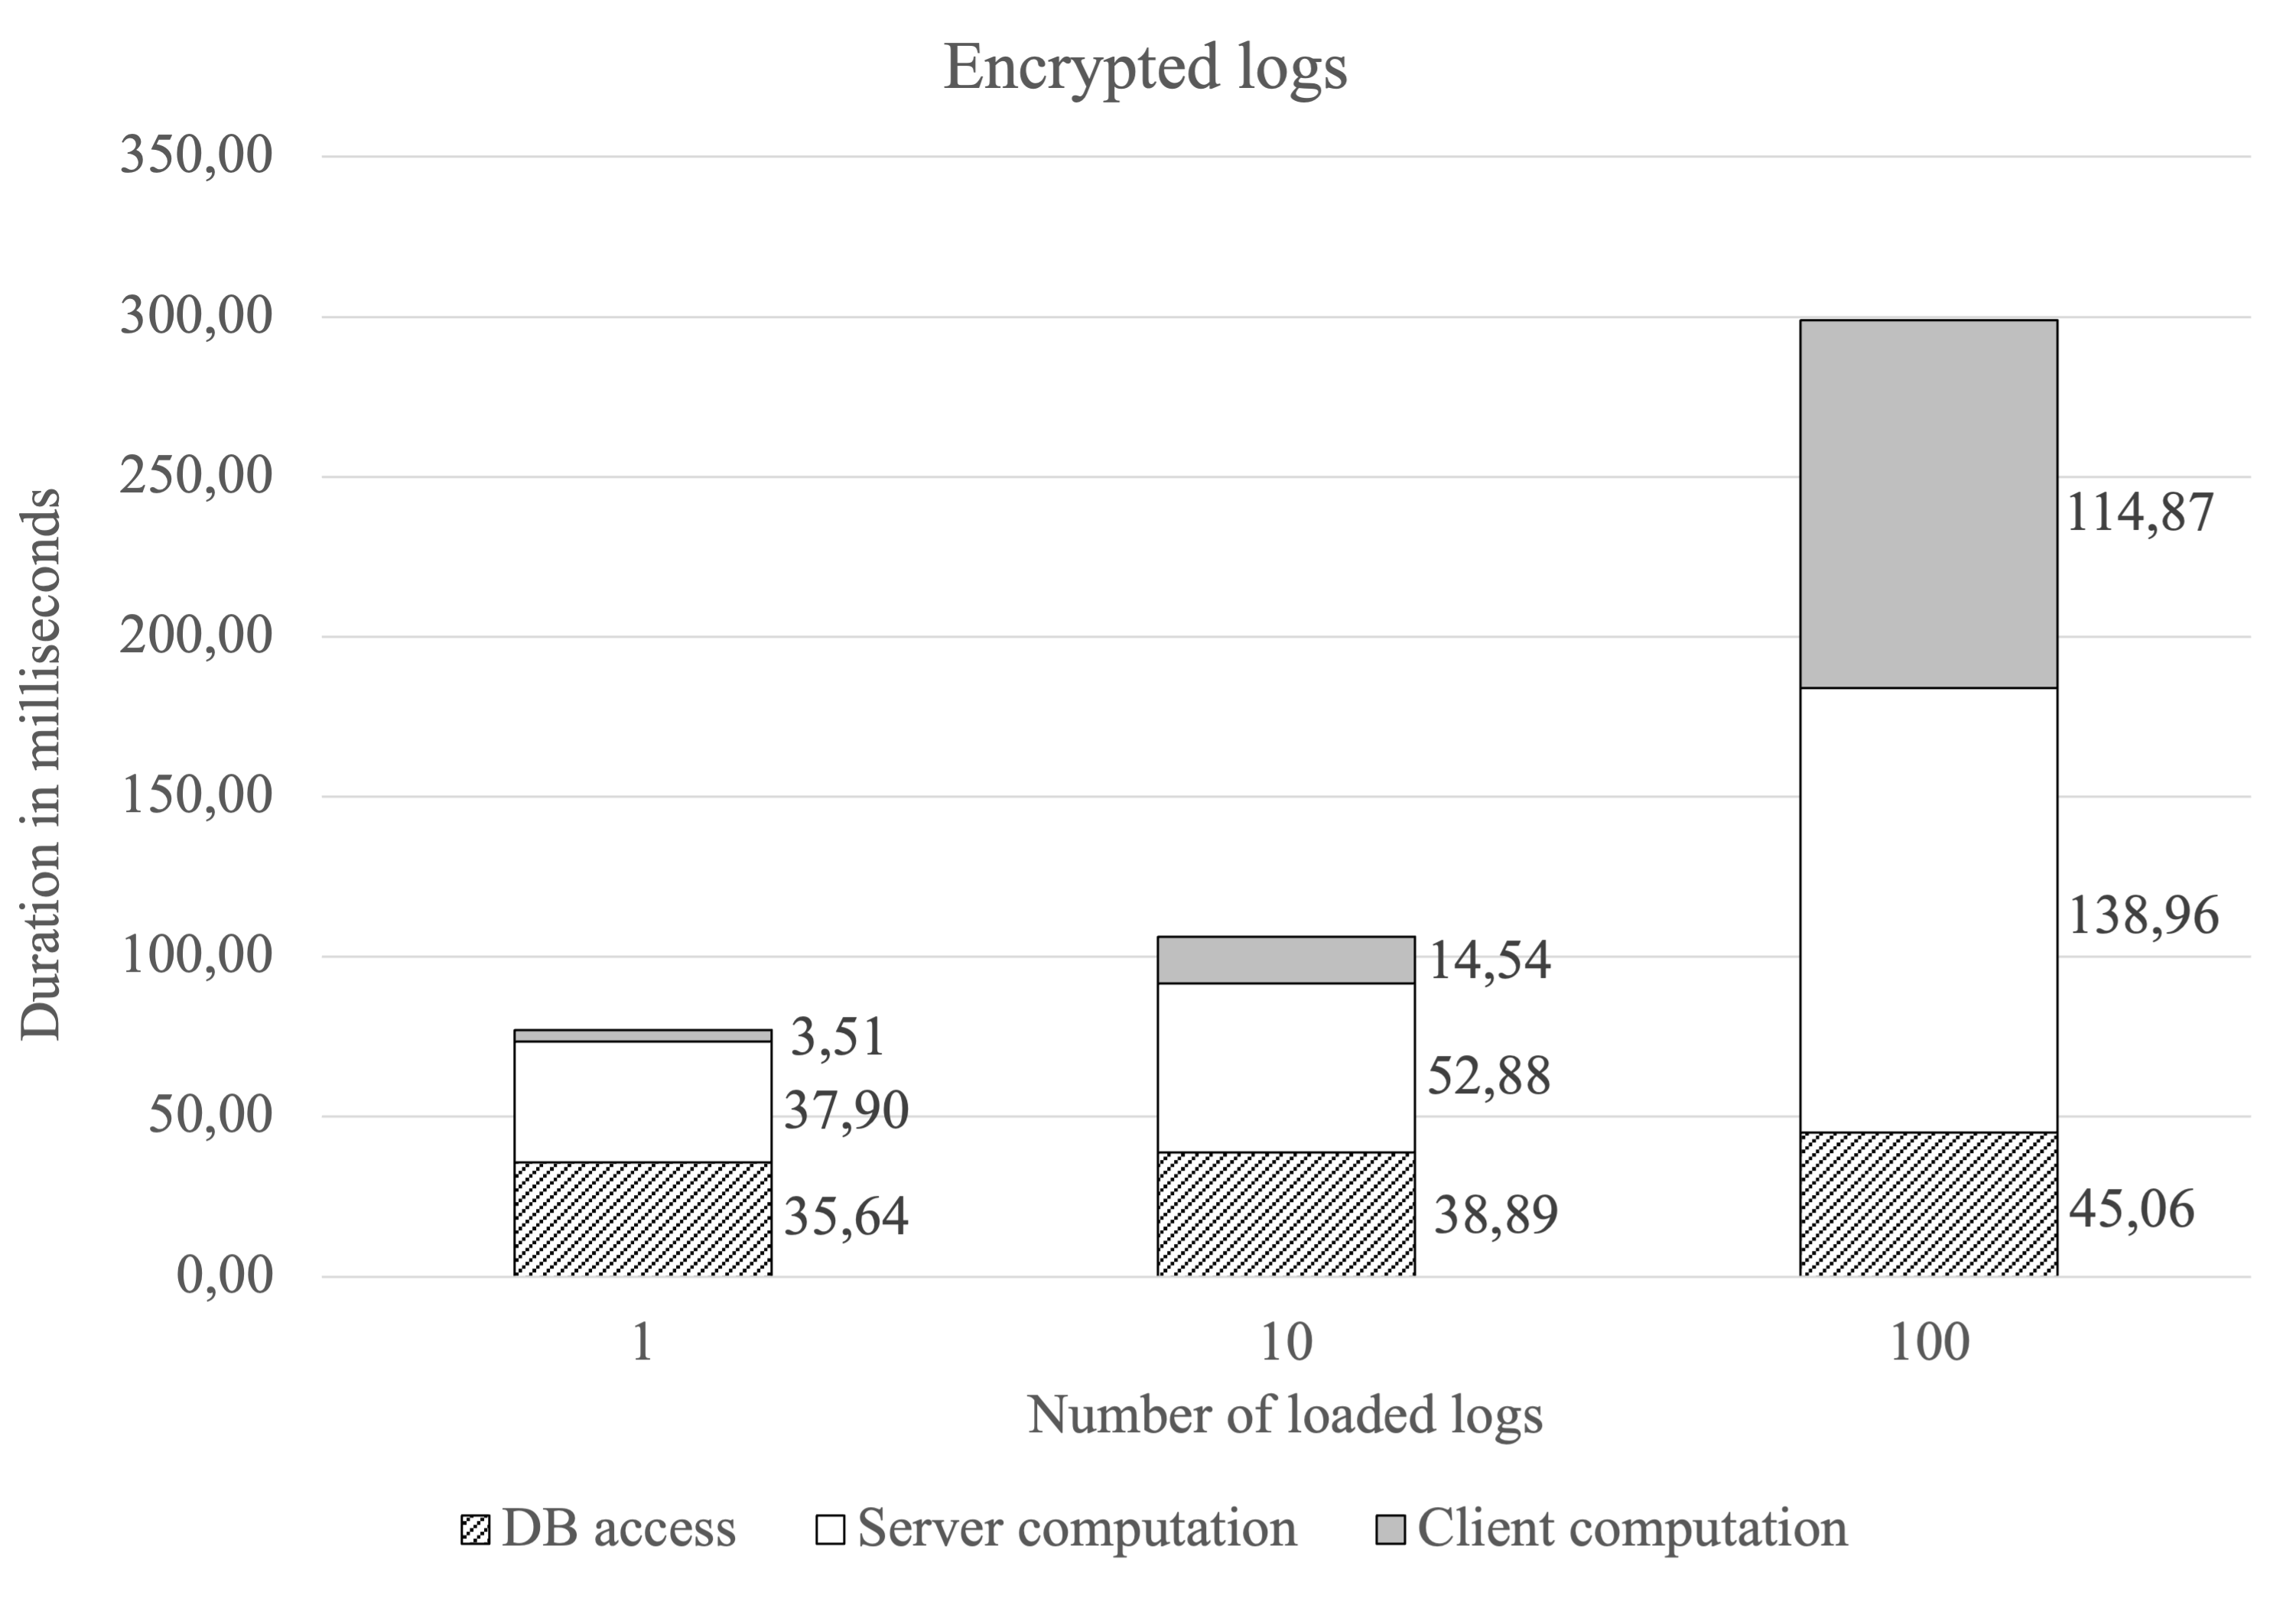
\includegraphics[scale=0.63]{../img/07/encrypted.png}
    \centering
    \caption[Measurements updated toolchain]{This figure visualizes the measured times to download and process the logs in the updated toolchain, which maintains encrypted logs.}
    \label{fig:perf-encrypted}
\end{figure}



\end{document}